%%%%%%%%%%%%%%%%%%%%%%%%%%%%%%%%%%%%%%%%%%%%%%%%%%%%%%%%%%%%%%%%%%%%%
%%                                                                 %%
%% Please do not use \input{...} to include other tex files.       %%
%% Submit your LaTeX manuscript as one .tex document.              %%
%%                                                                 %%
%% All additional figures and files should be attached             %%
%% separately and not embedded in the \TeX\ document itself.       %%
%%                                                                 %%
%%%%%%%%%%%%%%%%%%%%%%%%%%%%%%%%%%%%%%%%%%%%%%%%%%%%%%%%%%%%%%%%%%%%%

%%\documentclass[referee,sn-basic]{sn-jnl}% referee option is meant for double line spacing

%%=======================================================%%
%% to print line numbers in the margin use lineno option %%
%%=======================================================%%

%%\documentclass[lineno,sn-basic]{sn-jnl}% Basic Springer Nature Reference Style/Chemistry Reference Style

%%======================================================%%
%% to compile with pdflatex/xelatex use pdflatex option %%
%%======================================================%%

%%\documentclass[pdflatex,sn-basic]{sn-jnl}% Basic Springer Nature Reference Style/Chemistry Reference Style

%%\documentclass[sn-basic]{sn-jnl}% Basic Springer Nature Reference Style/Chemistry Reference Style
\documentclass[pdflatex,sn-mathphys]{sn-jnl}% Math and Physical Sciences Reference Style
\usepackage{array}
\usepackage{caption}
\usepackage[font=small]{caption}
\captionsetup{justification=centering}

%%\documentclass[sn-aps]{sn-jnl}% American Physical Society (APS) Reference Style
%%\documentclass[sn-vancouver]{sn-jnl}% Vancouver Reference Style
%%\documentclass[sn-apa]{sn-jnl}% APA Reference Style
%%\documentclass[sn-chicago]{sn-jnl}% Chicago-based Humanities Reference Style
%%\documentclass[sn-standardnature]{sn-jnl}% Standard Nature Portfolio Reference Style
%%\documentclass[default]{sn-jnl}% Default
%%\documentclass[default,iicol]{sn-jnl}% Default with double column layout

%%%% Standard Packages
%%<additional latex packages if required can be included here>
%%%%

%%%%%=============================================================================%%%%
%%%%  Remarks: This template is provided to aid authors with the preparation
%%%%  of original research articles intended for submission to journals published 
%%%%  by Springer Nature. The guidance has been prepared in partnership with 
%%%%  production teams to conform to Springer Nature technical requirements. 
%%%%  Editorial and presentation requirements differ among journal portfolios and 
%%%%  research disciplines. You may find sections in this template are irrelevant 
%%%%  to your work and are empowered to omit any such section if allowed by the 
%%%%  journal you intend to submit to. The submission guidelines and policies 
%%%%  of the journal take precedence. A detailed User Manual is available in the 
%%%%  template package for technical guidance.
%%%%%=============================================================================%%%%

\jyear{2022}%

%% as per the requirement new theorem styles can be included as shown below
\theoremstyle{thmstyleone}%
\newtheorem{theorem}{Theorem}%  meant for continuous numbers
%%\newtheorem{theorem}{Theorem}[section]% meant for sectionwise numbers
%% optional argument [theorem] produces theorem numbering sequence instead of independent numbers for Proposition
\newtheorem{proposition}[theorem]{Proposition}% 
%%\newtheorem{proposition}{Proposition}% to get separate numbers for theorem and proposition etc.

\theoremstyle{thmstyletwo}%
\newtheorem{example}{Example}%
\newtheorem{remark}{Remark}%

\theoremstyle{thmstylethree}%
\newtheorem{definition}{Definition}%

\raggedbottom
%%\unnumbered% uncomment this for unnumbered level heads

\begin{document}

\title[DNA Fingerprinting Lab]{Lab Report on DNA Fingerprinting}

\author*[1]{\fnm{Harsh} \sur{Agrawal}}\email{ha1822@ic.ac.uk}

\affil*[1]{\orgdiv{Molecular Bioengineering}, \orgname{Imperial College London}}
\affil*[1]{CID: 02320622}

% \abstract{The purpose of this lab was to carry out gel electrophoresis on DNA samples of different bacteria in order to identify an unknown bacteria using the same restriction enzyme. The report also discusses various underlying questions regarding the process and outcomes.}

\maketitle

\subsection*{Observation and Calculation}
\subsubsection*{Obtained Gel Image}
\begin{figure}[hp]
\centering
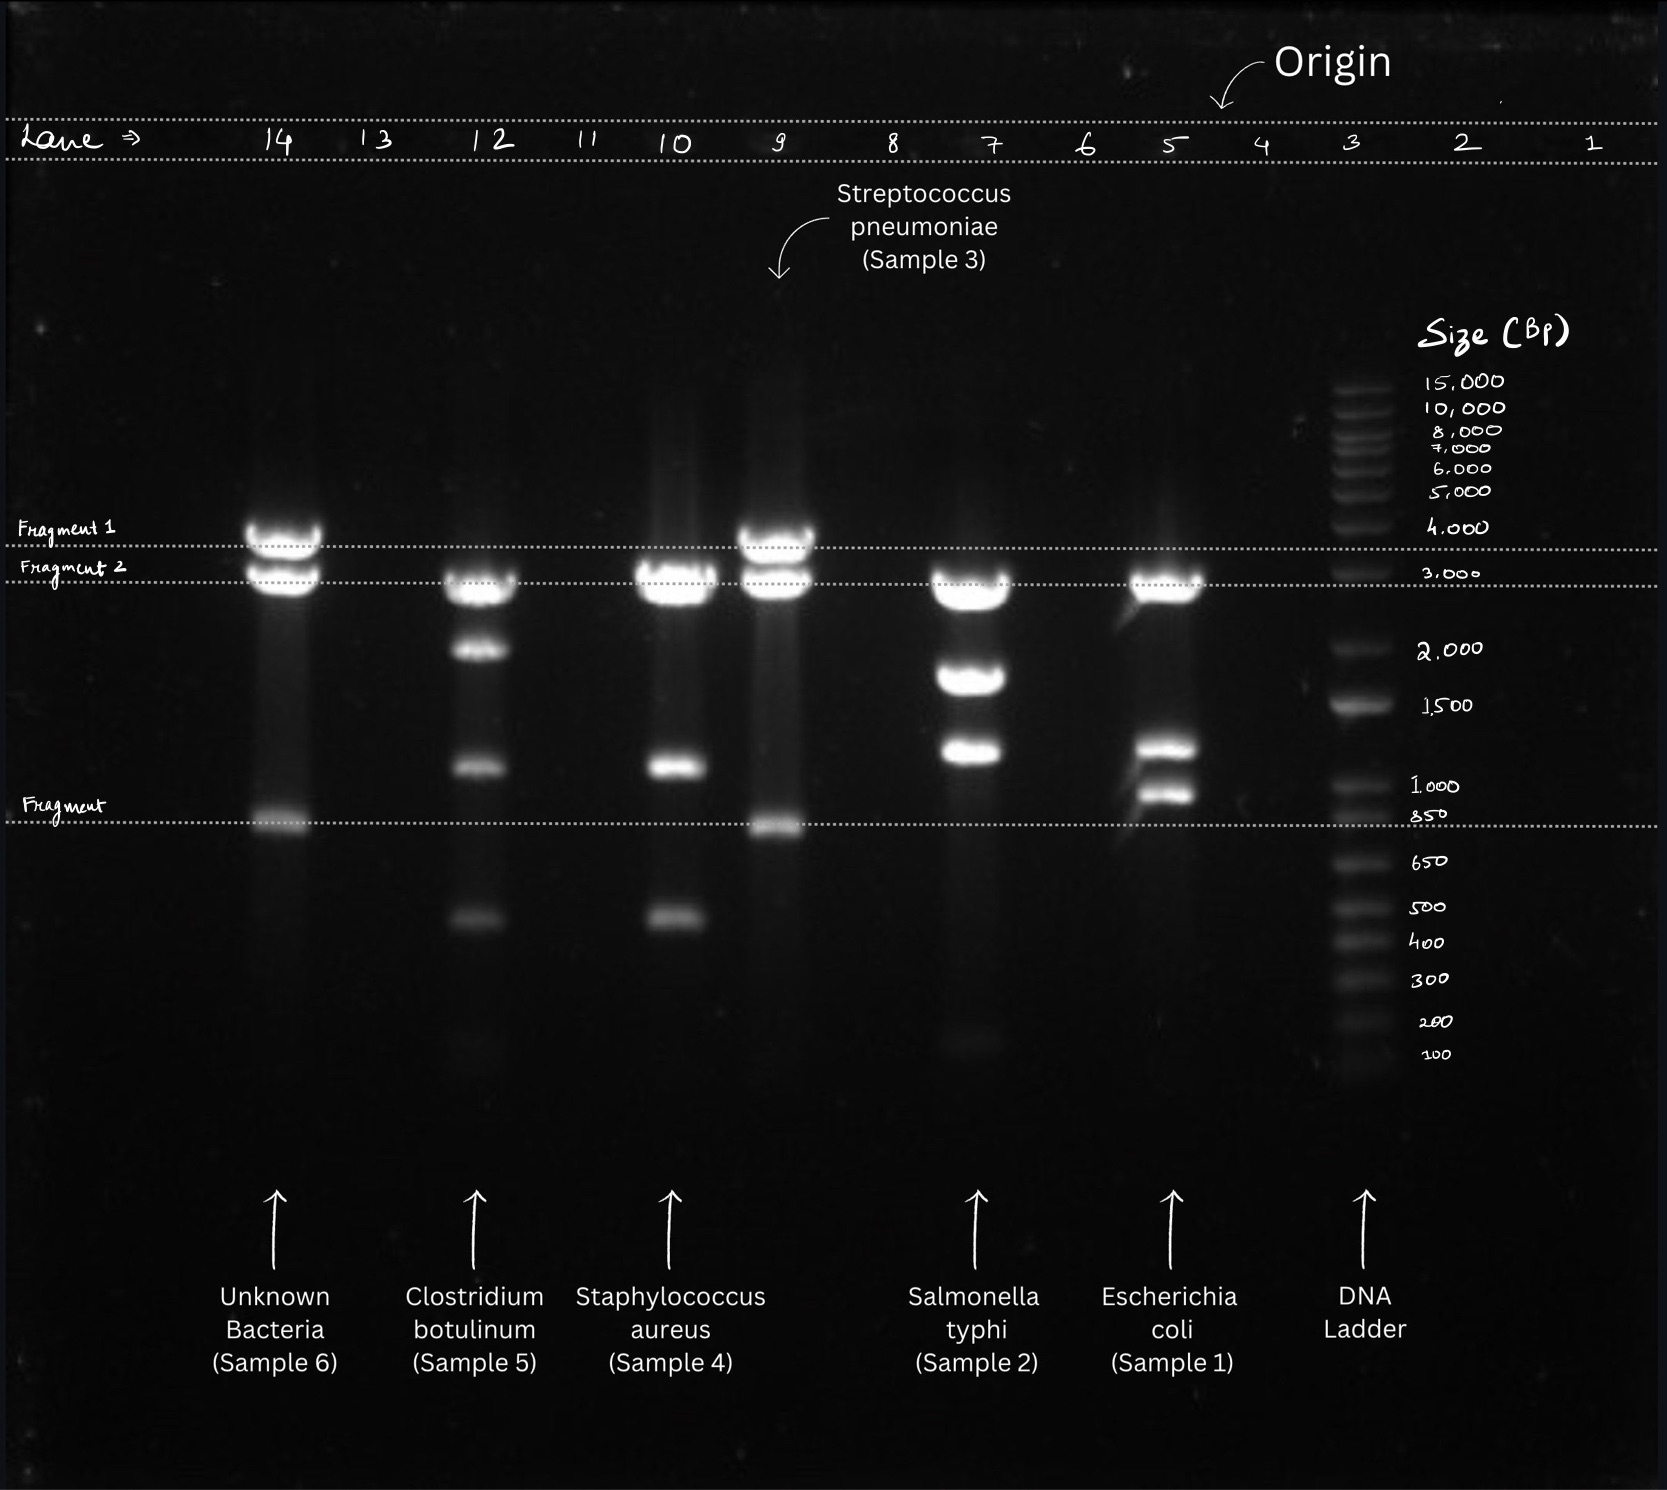
\includegraphics[width=0.8\textwidth]{photos/gelimage-3.jpg}
\caption{The following image was obtained after electrophoresis. The image is annotated with the origin, lanes, samples, and DNA ladder.}\label{fig1}
\end{figure}
From the following image, it can easily be observed that the DNA fragments of the unknown bacteria sample exactly match the DNA sample from the third bacteria sample. \vspace{7pt}

$\Rightarrow$ Unknown Bacteria = Streptococcus pneumonia (Sample 3).

\subsubsection*{Calculation of Fragment Weights}
To calculate the weights of the different fragments of the unknown bacteria, a calibration curve was plotted of distance traveled (in mm) of the DNA fragment against log\textsubscript{10}(base pairs) of the DNA ladder.

\begin{figure}[hp]
\centering
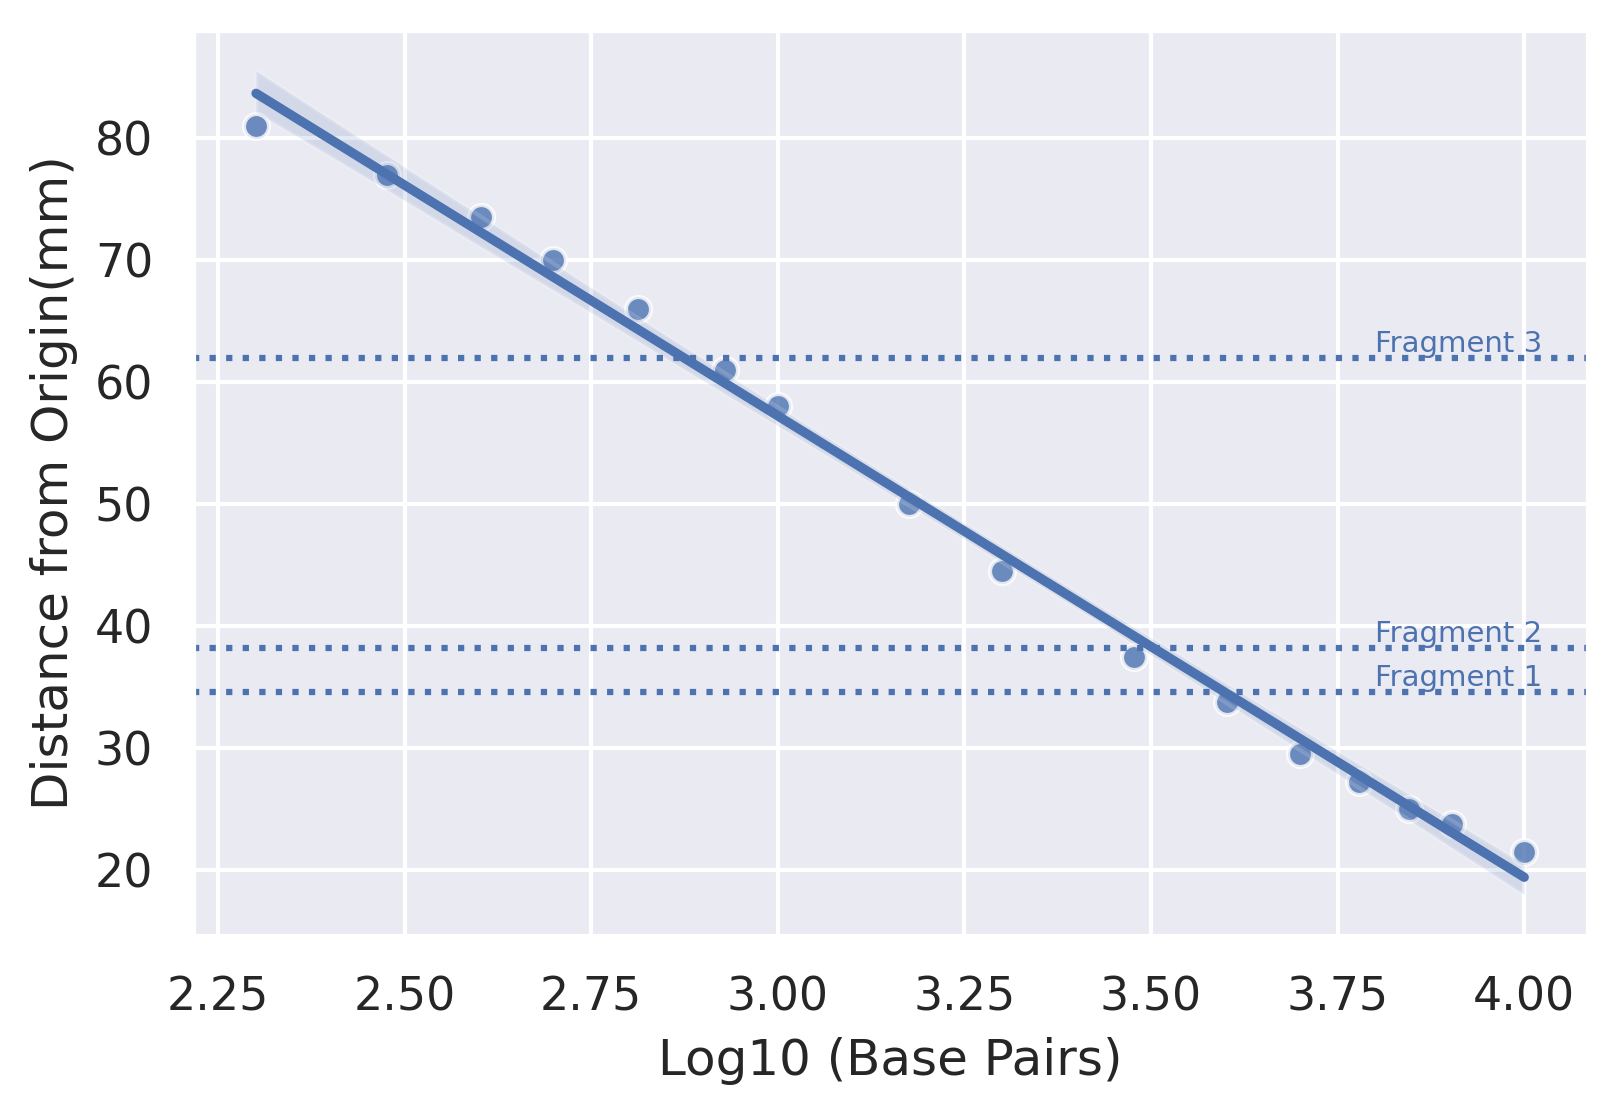
\includegraphics[width=1\textwidth]{photos/calibration curve.png}
\caption{The following calibration curve was obtained from the DNA ladder by estimating a line of best fit for the plotted points using the seaborn library in python.}\label{fig1}
\end{figure}
To obtain a better line of fit for the region underlying the unknown fragments, three points were excluded from both ends. The equation obtained for the updated line of best fit is:

\[y = -40.392x + 177.57\]
To calculate the weights (in Base Pairs) for the unknown fragments the distance traveled (in mm) was measured and plugged into the equation above. The following table summarizes the results obtained.
\begin{table}[h]
  \begin{center}
  \begin{minipage}{200pt}
  \caption{Velocity of Enzyme Activity vs pH}\label{tab1}
  \begin{tabular}{  m{5em}  m{5em} m{5em}  m{5em}} 
  % {@{\extracolsep{\fill}}lcccccc@{\extracolsep{\fill}}}
    \toprule
   Fragment Number & Distance Travelled (mm) & log\textsubscript{10}(base pairs) & Base Pairs.\footnotemark[1]\\
    \midrule
1. & 34.6 & 3.539 & 3464\\
2. & 38.2 & 3.450 & 2821\\
3. & 62 & 2.861 & 726\\
    \botrule
  \end{tabular}
\footnotetext[1]{Since the result is highly sensitive to the log\textsubscript{10} values, the accuracy of the calibration curve is vital. For a better fit, the distance calculation should be done via dedicated software(s) rather than manually.}
  \end{minipage}
  \end{center}
  \end{table}
\subsection*{Discussion}
\subsubsection*{1. Why do the samples go toward the positive electrode?}
\begin{figure}[hp]
\centering
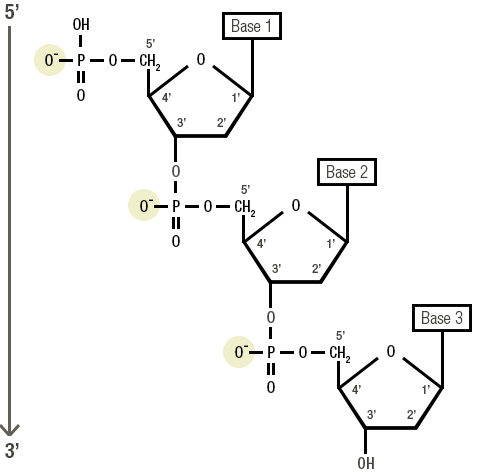
\includegraphics[width=0.5\textwidth]{photos/negative_charge_on_dna.png}
\caption{The following image was obtained from \href{https://elearning.fondation-merieux.org/molecular-biology/chapter-1/page-12.php}{https://elearning.fondation-merieux.org/molecular-biology/chapter-1/page-12.php}.}\label{fig1}
\end{figure}
DNA has a net negative charge due to the presence of the phosphate group. Due to this, when a voltage difference is applied across the ends of the gel, the DNA fragments move from the negatively charged electrodes to the positively charged electrodes via agarose. The lighter fragments travel farther than the heavier fragments.
\subsubsection*{2. Why are the bands a characteristic ‘smile’ shape?}
The bands appear to be a characteristic 'smile' shape as one visually-distinct fragment in the gel consists of multiple fragments of similar weights. The ends of the band consist of lighter sub-fragments that travel slightly farther than the bands present in the middle thus giving a 'smile' shape to the bands. This is a standard observation. 

However, if there is an appearance of a 'smile' shape across different lanes rather than in individual bands, then that might be caused due to the appliance of excessive voltage, uneven heating across the gel, or high sample concentrations. These factors can then be calibrated to obtain a better result. 

\subsubsection*{3. Why are the bands of different intensities? What implication does this have for DNA fingerprinting?}
The bands of different densities represent the respective amounts of DNA present in that fragment. The bands which are brighter and thicker contain a higher amount of DNA as compared to the bands which are dimmer or thinner. This could be highly useful in DNA fingerprinting as it can help analyze from different samples if the amount of DNA in two different samples is comparable and thus belong to the same individual.

\subsubsection*{4. Proteins can be separated by electrophoresis – called SDS-PAGE electrophoresis. Can you think or otherwise find out why they have to add sodium dodecyl sulphonate (SDS) to the sample to make this work?}
SDS-PAGE electrophoresis is a method commonly used to separate proteins with molecular masses between 5 and 250 kDa. Proteins are comprised of linear chains of 20 different amino acids. These naturally occurring amino acids bear neutral, net-negative, and net-positive charges. Thus the overall charge of proteins could vary heavily.

\begin{figure}[hp]
\centering
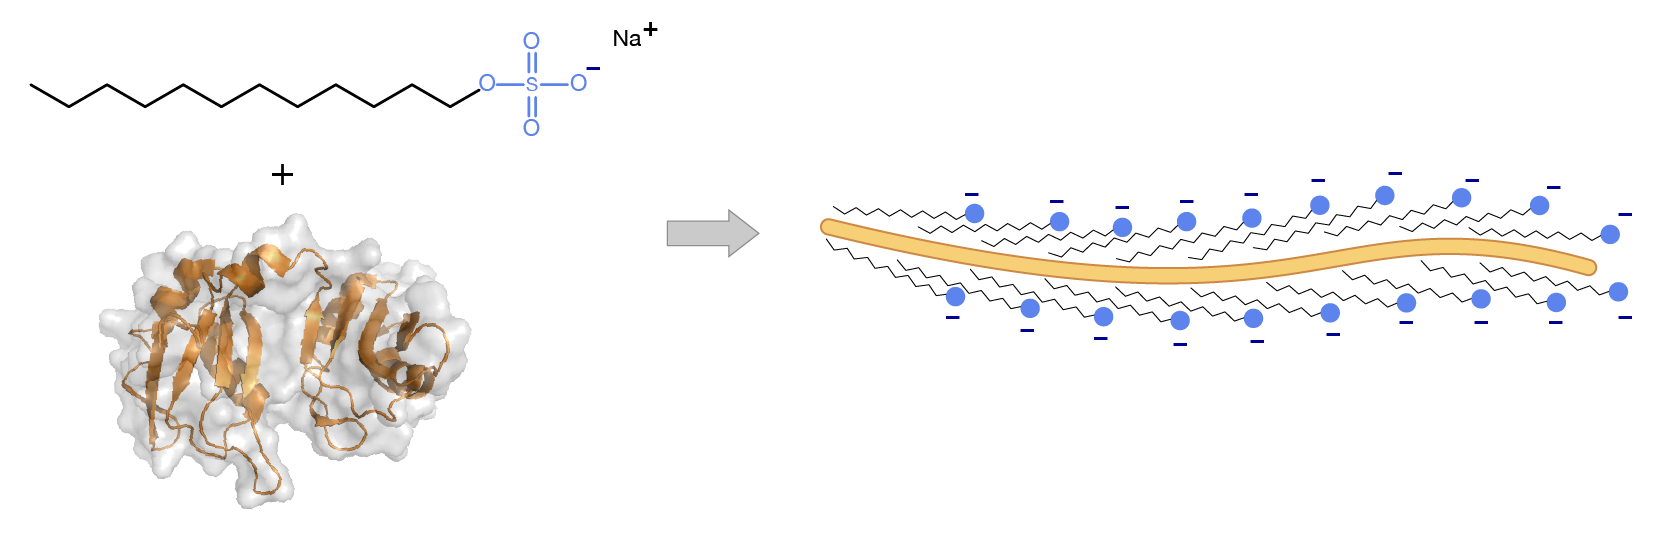
\includegraphics[width=0.8\textwidth]{photos/Protein-SDS_interaction.png}
\caption{The following image was obtained from \href{https://upload.wikimedia.org/wikipedia/commons/thumb/1/12/Protein-SDS_interaction.png/800px-Protein-SDS_interaction.png}{https://upload.wikimedia.org/wikipedia/commons/thumb/1/12/Protein-SDS-interaction.png}.}\label{fig1}
\end{figure}

To perform electrophoresis on proteins according to their molecular masses, these charges need to be masked. Thus, Sodium Dodecyl Sulphonate (SDS) is added as a surfactant that masks the intrinsic charge of proteins and provides it with a net-negative charge that allows them to move across the polyacrylamide gel. Without the application of SDS, the charge on proteins would interfere with the movement across the electric field. 

\end{document}
